\chapter{Le second principe de la thermodynamique} 
Ce principe exprime la conservation de l'énergie dans une transformation, 
sans faire de distinctions entre les énergies, ni dans le sens ou elles 
sont échangés. Pourtant, on sait que certaines transformations ne sont 
possible que dans un sens : ce principe nous permet de distinguer celles 
qui sont possibles.

	\section{Machines thermiques et réfrigérateurs}
	\begin{wrapfigure}[7]{l}{9cm}
	\vspace{-5mm}
	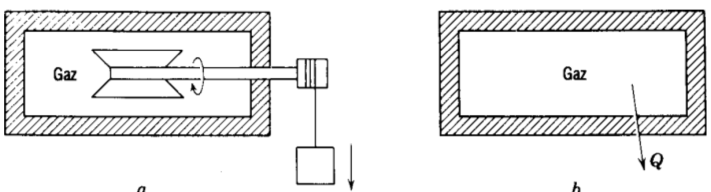
\includegraphics[scale=0.34]{ch6/image1.png}
	\captionof{figure}{ }
	\end{wrapfigure}
	Reconsidérons le système suivant en supposant que la transformation 
	comprenne  :
	\begin{enumerate}
	\item Un apport de travail sans échange de chaleur
	\item Refroidissement par transfert de chaleur
	\end{enumerate}
	Le cycle inverse est impossible, faire tourner le moteur ne le fera 
	au contraire par revenir à l'état initial : un corps froid recevant 
	de la chaleur devient chaud et ne deviendra pas froid par transfert 
	de chaleur vers le corps chaud.\\
	On introduit alors les notions de 
	\begin{description}
	\item[Machine thermique] Système décrivant un \textit{cycle moteur}, 
	c'est-à-dire recevant un travail net négatif (fourni du travail à 
	l'extérieur) et une chaleur nette positive résultant d'un échange de 
	chaleur provenant d'un corps chaud.
	\end{description}
	Dans un réfrigérateur, il faut recevoir de la chaleur d'un corps 
	froid : le travail net est positif $\Rightarrow$ chaleur nette 
	négative.\\
	
	\textsc{Exemple}. Considérons le cycle suivant 
	\begin{enumerate}
	\item On met une masse sur le piston en position la plus basse.
	\item On chauffe le gaz au maximum.
	\item On retire la masse
	\item On laisse refroidir
	\end{enumerate}
	Comme la masse a été soulevée, il s'agit bien d'un cycle moteur.\\
	
	\textsc{Exemple}. \\
	\begin{wrapfigure}[9]{r}{6cm}
	\vspace{-9mm}
	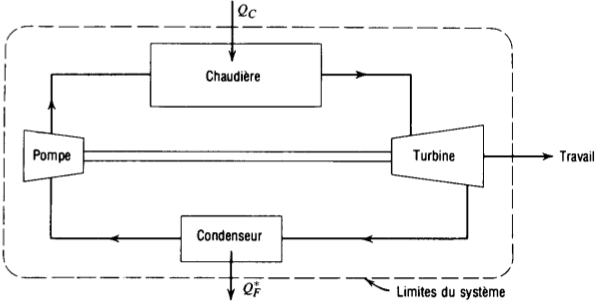
\includegraphics[scale=0.34]{ch6/image2.png}
	\captionof{figure}{ }
	\end{wrapfigure}
	Considérons la centrale thermique suivante. Ici, 
	c'est l'écoulement permanent d'une fluide qui décrit le cycle et 
	non plus une évolution cyclique temporelle.\\
	Introduisons l'\textbf{efficacité thermique}\footnote{Rendement 
	thermique.} comme le rapport de l'\textit{effet utile} (ici, le 
	travail) à l'\textit{effet onéreux} (ici, la chaleur reçue par 
	le corps chaud\footnote{On ne compte pas la chaleur cédée au corps 
	froid.}) :
	\begin{equation}
	\varepsilon_{th} = \frac{W^*}{Q_C} = \frac{Q_C-Q_F^*}{Q_C} = 1-
	\frac{Q_F^*}{Q_C} <1
	\end{equation}
	Considérons maintenant un système de réfrigération. L'efficacité 
	dépend de l'effet utile recherché. Si on s'intéresse à extraire 
	la chaleur d'un corps froid (le coefficient de performance) (%
	fonctionnement en réfrigérateur) :
	\begin{equation}
	\varepsilon_{fr} = \frac{Q_F}{W} = \frac{Q_F}{Q_C^*-Q_F} = \frac{
	1}{Q_C^*/Q_F-1}
	\end{equation}
	Si on s'intéresse  à la chaleur cédée au corps chaud (pompe à 
	chaleur) : 
	\begin{equation}
	\varepsilon_{ch} = \frac{Q_F}{W}=\frac{Q_C^*}{Q_C^*-Q_F}=\frac{1}{
	1-Q_F/Q_C^*} = 1+\epsilon_{fr} >1
	\end{equation}
	Tout ceci est possible grâce aux \textbf{réservoirs thermiques} : 
	il s'agit d'un système susceptible d'échanger une quantité 
	quelconque de chaleur sans que sa température soit modifiée.
	
	
	\section{Le second principe de la thermodynamique}
	Deux formulations équivalentes existent : celle de Kelvin-Planck 
	et celle de Clausius. 
	
	\proposition{Il est impossible de réaliser un appareil décrivant 
	un cycle qui fournit du travail en échangeant de la chaleur 
	avec une seule source.}\ \\
	On se réfère aux machines thermiques : on ne peut transformer 
	totalement en travail la chaleur reçue d'une source chaude\\
	
	\proposition{Il est impossible de réaliser un appareil décrivant 
	un cycle dont le seul effet serait de transférer une quantité 
	de chaleur d'une source froide à une source chaude.}\ \\
	On se réfère aux machines frigorifiques, car on ne peut en 
	réaliser une sans apport de travail.
	
		\subsection{Équivalence des énoncés} 
		On va montrer que l'énoncé de Clausius entraîne celui de 
		Kelvin-Planck.
		
		\begin{proof}\ \\
		Supposons qu'on puisse créer un appareil transférant $Q_F$ 
		d'une source froide à chaude sans $W$ et associons-y une 
		machine thermique produisant un travail $W=Q_C-Q_F$ en 
		recevant $Q_C$ de la source chaude et en rejetant $Q_F$ à la source froide. 
		Le système composé des deux machines et de la source 
		froide fourni du travail en échangeant de la chaleur avec 
		seulement la source chaude, ce qui viole Kelvin-Planck.
		
		\begin{center}
		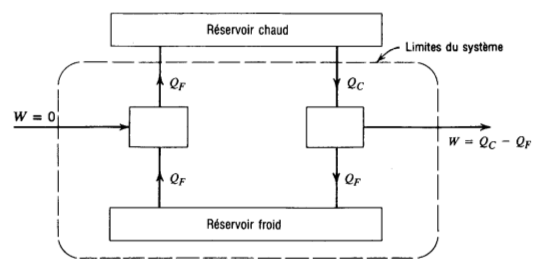
\includegraphics[scale=0.5]{ch6/image3}
		\captionof{figure}{Équivalence des énoncés}
		\end{center}
		\end{proof}
		
		\subsection{Impossibilité des mouvements perpétuels}
		Comme il est impossible de transférer intégralement une 
		quantité de chaleur en travail, il est impossible de créer 
		un \textbf{mouvement perpétuel de deuxième espèce} : un 
		système produisant du travail en puisant dans une source 
		"gratuite".
		
		\subsection{Classification et dégradation de l'énergie}
		Un travail peut etre intégralement transformé en chaleur, 
		l'inverse est faux : le travail est "plus noble". De plus 
		la chaleur cédée à la source froide par une machine 
		thermique n'est pas la même que celle puisée à la source 
		froide car elle ne peut plus être transformée en travail : 
		l'énergie est dégradée.


	\section{Les transformations réversibles}
	Comme $\varepsilon_{th} < 1$, il serait cool de savoir pour quel système
	l'efficacité tend vers 1. Définissons d'abord :
	\begin{description}
	\item[Transformation réversible] Une transformation est 
	réversible lorsqu'elle peut être décrite en sens inverse de 
	sorte qu'après avoir été décrite dans les deux sens de façon 
	successive, tant le système considéré que le milieu extérieur 
	est dans le même état qu'initialement.
	\end{description}
	Pour être réversible, il faut que durant la transfo. inverse :
	\begin{enumerate}
	\item Les variables d'états repassent par les même valeurs que 
	pour la transfo. initiale.
	\item Les échanges d'énergies soient exactement opposés.
	\end{enumerate}
	
	
	\section{Les sources d'irréversibilité}
		\subsection{Les frottements}
		Ils transforment le travail en chaleur, par nature 
		irréversible.
		
		\subsubsection{La détente libre}
		Irréversible car on ne peut ramener le travail dans son 
		état initial que par apport de travail et cession de 
		chaleur.
		
		\subsection{L'échange de chaleur entre deux sources}
		Supposons que de la chaleur soit transférée d'une source 
		chaude à froide, transfo irréversible (Clausius) : il 
		ne peut exister de transfert de chaleur réversible qu'entre 
		deux sources de différence de température infinitésimale.
	
	
	\section{Le cycle de Carnot}
	\begin{wrapfigure}[9]{l}{7.5cm}
	\vspace{5mm}
	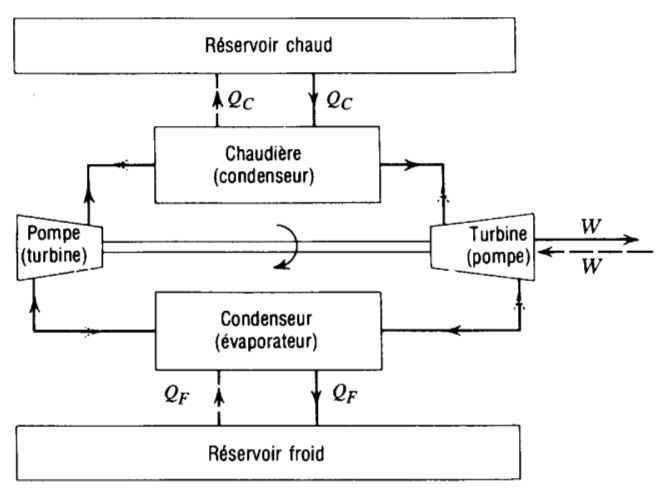
\includegraphics[scale=0.34]{ch6/image4.png}
	\captionof{figure}{ }
	\end{wrapfigure}
	Une machine fonctionnant entre source chaude et froide décrivant 
	un cycle dont toutes les transformations sont réversible est un 
	\textbf{cycle de Carnot}, le best cycle ever. Il se comporte de :
	\begin{enumerate}
	\item Dans la chaudière, on reçoit du $Q$ : la température du fluide 
	doit être la même que celle de la source chaude comme l'échange de chaleur
	doit être réversible, transformation \textbf{isotherme réversible}.
	\item Dans la turbine, il subit une détente \textbf{adiabatique réversible} 
	en fournissant un travail : diminution de $T$ jusqu'à la température 
	de la source froide.
	\item Dans le condenseur il cède de la chaleur à la source froide : 
	\textbf{isotherme réversible}.
	\item Compression \textbf{adiabatique réversible} dans le compresseur : $T$ 
	augmente jusqu'à la température de la source chaude.
	\end{enumerate}\ 
	\begin{center}
		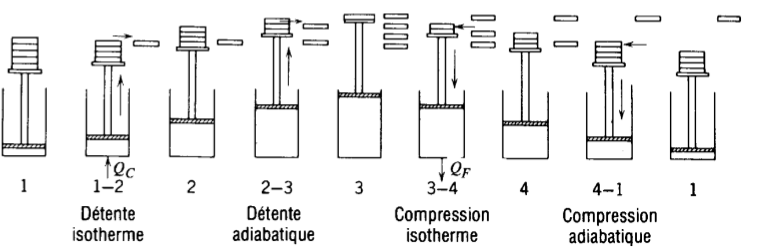
\includegraphics[scale=0.34]{ch6/image5.png}
	\captionof{figure}{Représentation possible d'un cycle de Carnot}
	\end{center}
	
	\section{Deux propriétés des cycles de Carnot}
	\proposition{Il est impossible de réaliser une machine 
	fonctionnant entre deux sources qui serait plus efficace qu'une 
	machine réversible fonctionnant entre les deux même sources.}\ \\
	Par l'absurde, supposons qu'une telle machine (ici thermique) 
	existe. Soit $Q_C$ la chaleur reçue à la source chaude et $W_{M.I}^*$ 
	le travail fourni supposé plus grand que $W_{M.R.}^*$, le travail 
	fourni par la machine réversible recevant la même $Q_C$.\\
	Le système formé de la machine irréversible hypothétique, de la 
	machine réversible fonctionnant en sens inverse et de la source 
	chaude viole Kelvin-Planck.
	
	\begin{center}
	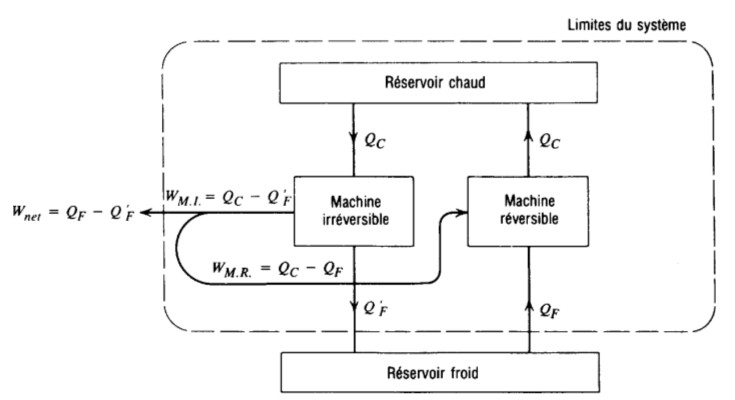
\includegraphics[scale=0.4]{ch6/image6.png}
	\captionof{figure}{Preuve de la première proposition}
	\end{center}
	
	\proposition{Toutes les machines décrivant un cycle de Carnot entre 
	deux sources ont la même efficacité.}\ \\
	Se démontre semblablement.
	
	
	\section{L'échelle de température thermodynamique}
	\begin{wrapfigure}[10]{l}{5cm}
	\vspace{-5mm}
	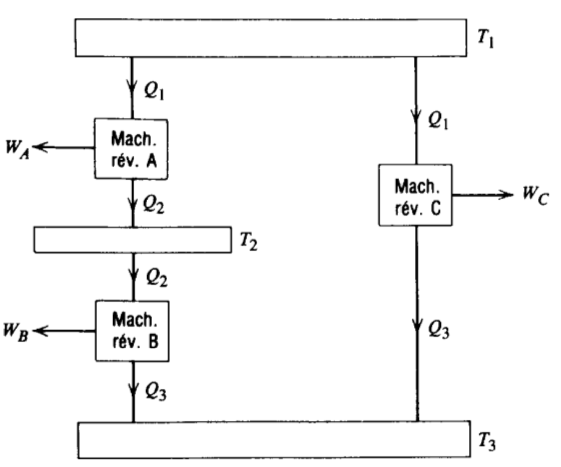
\includegraphics[scale=0.25]{ch6/image7.png}
	\captionof{figure}{ }
	\end{wrapfigure}
	Comme tous les cycles ont la même efficacité, celle-ci ne peut 
	dépendre que des températures des sources. Cela s'écrit 
	\begin{equation}
	(\varepsilon_{th})_{Carnot} = 1-\frac{Q_F^*}{Q_C} = 1 - 
	\psi(T_F,T_C)
	\end{equation}
	où $T_C,T_F$ sont les températures des sources dans l'échelle 
	absolue à définir.\\
	Soit trois sources de températures $T_1,T_2$ et $T_3$ telles que 
	$T_1 > T_2 > T_3$ avec les cycles de Carnot pris deux à deux.\\
	On a :\vspace{3mm}
	\begin{equation}
	1-\varepsilon_{th,A} = \frac{Q_2}{Q_1} = \psi(T_2,T_1),\quad 
	1-\varepsilon_{th,B} = \frac{Q_3}{Q_2} = \psi(T_3,T_2),\quad 
	1-\varepsilon_{th,C} = \frac{Q_3}{Q_1} = \psi(T_3,T_1),\quad 
	\end{equation}
	Il en résulte que
	\begin{equation}
	\psi(T_2,T_1)\psi(T_3,T_2) = \psi(T_3,T_1)
	\end{equation}
	La fonction $\psi(x,y)$ doit forcément être de la forme $f(x)/
	f(y)$ et donc d'après la définition
	\begin{equation}
	\frac{Q_F^*}{Q_C} = \frac{f(T_F)}{f(T_C)}
	\end{equation}
	$f$ est forcément de signe constant et croissante car $\frac{Q_3}{
	Q_1}<\frac{Q_2}{Q_1}$. Si $f$ vérifie ceci, alors on peut l'utiliser 
	comme échelle absolue. On choisi la forme linéaire $f = \alpha T$. 
	Pour choisir $\alpha$ on peut faire en sorte que la différence de 
	température soit identique à sa valeur dans une échelle conventionnelle 
	choisie. Si $T_1=0$ et $T_2=100^\circ C$, l'efficacité du cycle de 
	Carnot est de $0.268$ de sorte que $T_{glace} = 273.15\ K$. Comme $f$
	doit être de signe constant, elle ne peut devenir négative d'où la 
	notion de \textbf{zéro absolu}. Voir les deux derniers slide pour savoir 
	comment mesurer la température thermodynamique à l'aide d'un thermomètre 
	à gaz à volume constant.
